% !TeX root = ../libro.tex
% !TeX encoding = utf8

\chapter{Conceptos básicos}

\begin{definicion} Una \textbf{primitiva} es el objeto básico de visualización. Pueden ser puntos, segmentos, patrones de segmentos, polígonos y patrones de polígonos. En nuestro caso las primitivas a usar serán triángulos.
\end{definicion}

\begin{definicion} Entenderemos por \textbf{malla} una malla de triángulos, que es un conjunto de triángulos que aproximan a una cierta superficie. Cuando nos referimos a la malla inicial, hablamos de la aproximación del cuadrado $[0,1]\times[0,1]\subset \R^2$ para un cierto número de triángulos (se calcula una cuadrícula y se dividen por las diagonales para obtener los triángulos).
\end{definicion}

\begin{definicion} La acción \textbf{teselar} consiste en subdividir una primitiva en primitivas más pequeñas, para así poder aproximar mejor la superficie que se quiere representar. En el caso de OpenGL, para realizar la teselación es necesario especificar los respectivos niveles de teselado.
\end{definicion}

\begin{definicion} El \textbf{nivel de teselado en un lado} (outer) es el número de partes en el que se dividirá el lado para el teselado de la primitiva. Por ejemplo, si el nivel es $3$ para un cierto lado, dicho lado se dividirá en $3$ partes iguales, que serán los lados de los nuevos triángulos.
\end{definicion}

\begin{definicion} El \textbf{nivel de teselado en el interior} (inner) es el número de partes en el que se dividirá la primitiva hacia el interior. Por ejemplo, si el nivel es $3$ para una cierta primitiva, dicha primitiva se dividirá en $3$ niveles hacia el baricentro.
\end{definicion}

\begin{figure}[h]
  	\centering
  	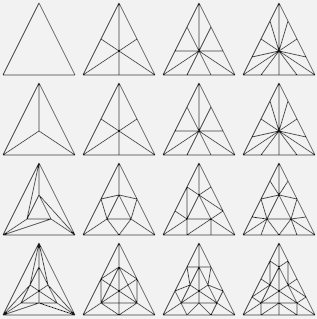
\includegraphics[width=0.4\textwidth]{nivel_tess}
	\caption{Niveles de teselado del $1$ al $4$: outer en horizontal (todos los lados por igual) e inner en vertical.}
  	\label{fig:nivel_tess}
\end{figure}

\begin{definicion} Un \textbf{shader} es un tipo específico de programa informático que se ejecuta en la GPU. Su uso principal es el cálculo de gráficos. En OpenGL existen los siguientes tipos de shaders:
	\begin{itemize}
		\item Vertex shader: se ejecuta para cada vértice de entrada. Se utiliza para podificar cada vértice.
		\item Tessellation control shader: tiene de entrada una primitiva y devuelve un patch (conjunto de primitivas), según los niveles de teselado.
		\item Tessellation evaluation shader: similar al vertex shader pero diseñado para la salida del tessellation control shader.
		\item Geometry shader: tiene de entrada una primitiva y devuelve varias primitivas.
		\item Fragment shader: después del rasterizado (pasar de gráfico vectorial a píxels), se ejecuta para calcular el color de cada fragmento de triángulo.
		\item Compute shader: etapa utilizada para realizar cáculos en general. No suele usarse para el renderizado en sí (no se ha utilizado en el proyecto).
	\end{itemize}
\end{definicion}

\begin{definicion} La \textbf{curvatura de Gauss} (K) es una función que a cada punto de una superficie $S$ le asigna un valor de $\R$. Indica el tipo de geometría entorno al punto:
	\begin{itemize}
		\item $K_p = 0$, euclídea, localmente es $\R^2$.
		\item $K_p > 0$, esférica, localmente es una esfera de radio $R = \frac{1}{\sqrt{K_p}}$.
		\item $K_p < 0$, hiperbólica, localmente es un espacio hiperbólico de cruvatura $K_p$.
	\end{itemize}
La curvatura de Gauss se ha calculado de la siguiente forma (CITAR WOLFRAM):
		$$K_{x(u,v)} = \frac{det(x_{uu}, x_u, x_v) det(x_{vv}, x_u, x_v) - [det(x_{uv}, x_u, x_v)]^2} {[|x_u|^2|x_v|^2 - <x_u, x_v>^2]^2} (u, v)$$
	que es la curvatura de Gauss en el punto $x(u, v)$, con $x$ carta de la superficie $S$. Existen muchas maneras distintas de calcularla, pero esta es la que nos favorecerá para su correcta obtención mediante los árboles de expresión.
\end{definicion}

\endinput
%------------------------------------------------------------------------------------
% FIN DEL CAPÍTULO. 
%------------------------------------------------------------------------------------
